\documentclass[10pt]{beamer}
% options: draft, compress, handout
\usepackage{amsmath,amssymb,amsfonts,textcomp,amsthm,xifthen,psfrag,graphicx,color,MnSymbol}
\usepackage{multicol}
\usepackage[T1]{fontenc}
\usepackage{svg}
\usefonttheme{serif}
\mode<presentation>
{
  \usetheme{AnnArbor} % not bad at all, rel. simple, sleek design
  \setbeamercovered{transparent}
  %gets rid of bottom navigation bars
  %\setbeamertemplate{footline}[page number]{}   % page number
  \setbeamertemplate{footline}[frame number]{}   % frame number
  %gets rid of navigation symbols
  \setbeamertemplate{navigation symbols}{}
  \setbeamercolor{block title}{bg=blue!30,fg=blue}
}
%\usepackage{appendixnumberbeamer}
%\oddsidemargin 0.5cm
%\textwidth     16cm
%\textheight    20cm
%\setlength\parindent{0pt}

%\newtheorem{theorem}{Teorema}
\newtheorem{cor}[theorem]{Corolario}
\newtheorem{prop}[theorem]{Proposición}
\newtheorem{remark}[theorem]{Nota}
\newtheorem{hip}[theorem]{Hipótesis}

\newtheorem{algorithm}[theorem]{Algoritmo}

%
\newcommand{\ndof}{\#\mathrm{dof}}
%----------------------------------------------------------------------------------
\DeclareFontFamily{U}{matha}{\hyphenchar\font45}
\DeclareFontShape{U}{matha}{m}{n}{
      <5> <6> <7> <8> <9> <10> gen * matha
      <10.95> matha10 <12> <14.4> <17.28> <20.74> <24.88> matha12
      }{}
\DeclareSymbolFont{matha}{U}{matha}{m}{n}
\DeclareFontSubstitution{U}{matha}{m}{n}

% Math symbol font mathb
\DeclareFontFamily{U}{mathx}{\hyphenchar\font45}
\DeclareFontShape{U}{mathx}{m}{n}{
      <5> <6> <7> <8> <9> <10>
      <10.95> <12> <14.4> <17.28> <20.74> <24.88>
      mathx10
      }{}
\DeclareSymbolFont{mathx}{U}{mathx}{m}{n}
\DeclareFontSubstitution{U}{mathx}{m}{n}

% Symbol definition
\DeclareMathDelimiter{\vvvert}{0}{matha}{"7E}{mathx}{"17}



%-------------------------------------------------------------------------------
\newcommand{\<}{\langle{}}
\renewcommand{\>}{\rangle}
\newcommand{\ip}[2]{\llangle#1\hspace*{.5mm},#2\rrangle}
\newcommand{\dual}[2]{\<#1\hspace*{.5mm},#2\>}
\newcommand{\dualg}[2]{\<#1\hspace*{.5mm},#2\>^\nabla}
\newcommand{\duald}[2]{\<#1\hspace*{.5mm},#2\>^\mathrm{div}}
\newcommand{\dualgd}[2]{\<#1\hspace*{.5mm},#2\>^{\nabla\mathrm{div}}}
\newcommand{\dualcc}[2]{\<#1\hspace*{.5mm},#2\>^{\Curl^2}}
\newcommand{\dualgg}[2]{\<#1\hspace*{.5mm},#2\>^{\Grad\grad}}
\newcommand{\dualdd}[2]{\<#1\hspace*{.5mm},#2\>^{\Div\div}}
\newcommand{\dualgc}[2]{\<#1\hspace*{.5mm},#2\>^{\Grad\Curl}}
\newcommand{\dualgca}[2]{\<#1\hspace*{.5mm},#2\>^{\GCurla}}
\newcommand{\dualRM}[3]{\<#1\hspace*{.5mm},#2\>_{#3}}
\newcommand{\vdual}[2]{(#1\hspace*{.5mm},#2)}
%\newcommand{\abs}[1]{\vert #1 \vert}
%\newcommand{\norm}[2]{\|#1\|_{#2}}
%\newcommand{\snorm}[2]{|#1|_{#2}}

\renewcommand{\skew}[1]{\mathrm{skew}(#1)}
\newcommand{\diam}{\mathrm{diam}}
\newcommand{\wilde}{\widetilde}
\newcommand{\wat}{\widehat}
\newcommand{\transp}{\mathsf{T}}

\newcommand{\cQ}{{c_Q}}
\newcommand{\cQinv}{{c_Q^{-1}}}
\newcommand{\Cdisp}{{\mathbf{C}_\mathrm{disp}}}
\newcommand{\Cdispt}{{\mathbf{C}_\mathrm{disp}^2}}
\newcommand{\Cdispinv}{{\mathbf{C}_\mathrm{disp}^{-1}}}
\newcommand{\Cdispinvt}{{\mathbf{C}_\mathrm{disp}^{-2}}}
\newcommand{\cdisp}{{c_\mathrm{disp}}}
%\newcommand{\cdefl}{c_\mathrm{defl}}

\newcommand{\Grad}{\boldsymbol{\nabla}}
\newcommand{\sGrad}{\boldsymbol{\varepsilon}}
\newcommand{\kGrad}{{\boldsymbol{\nabla}'}}
\newcommand{\pwkGrad}{{\boldsymbol{\nabla}_\cT'}}
\def\pwGrad{\boldsymbol{\nabla}_\cT}
\def\pwsGrad{\boldsymbol{\varepsilon}_\cT}
\def\Div{{\rm\bf Div\,}}
\def\pwDiv{{\rm\bf div}_\cT}
\def\grad{\nabla}
\def\pwgrad{\nabla_\cT}
\def\GG{\mathbf{G}}
\def\MM{\mathbf{M}}
\def\SS{\mathbf{S}}
\def\BB{\mathbf{B}}
\def\DD{\mathbb{D}}
\def\NN{\mathbf{N}}
\def\TT{\mathbf{T}}
\def\WW{\mathbf{W}}
\def\ZZ{\mathbf{Z}}
\def\II{\mathbf{I}}
\def\QQ{\mathbf{Q}}
\def\PP{\mathbf{P}}
\def\KK{\mathbf{K}}
\def\bQ{\mathbf{Q}}
\newcommand{\bC}{\boldsymbol{\mathcal{C}}}
\newcommand{\CC}{\boldsymbol{C}}
\def\bR{\boldsymbol{R}}
\def\TTheta{\mathbf{\Theta}}
\def\bq{\boldsymbol{q}}
\def\rr{\mathbf{r}}
\def\bz{\boldsymbol{z}}
\def\Amat{\boldsymbol{A}}
\def\Bmat{\boldsymbol{B}}
\def\Cmat{\boldsymbol{C}}

\newcommand{\cRT}{\mathcal{RT}}
\newcommand{\cL}{\ensuremath{\mathcal{L}}}
\newcommand{\bL}{\ensuremath{\boldsymbol{L}}}
\newcommand{\LL}{\ensuremath{\mathbb{L}}}
%\def\tQ{\wat{\boldsymbol{q}}}
\def\tq{\wat{\boldsymbol{q}}}
%\def\tT{\wat{\boldsymbol{\theta}}}
\def\btheta{\boldsymbol{\theta}}
\def\bbeta{\boldsymbol{\beta}}
\def\bkappa{\boldsymbol{\kappa}}
\def\CDiv{\mathrm{CDiv}}
\DeclareMathOperator{\GCurl}{\Grad\Curl}
\DeclareMathOperator{\rot}{rot}
\DeclareMathOperator{\Rot}{{\bf rot}}
\DeclareMathOperator{\scurl}{\mathrm{sym}\curl}


\DeclareMathOperator{\aGrad}{\boldsymbol{\nabla^{\textmd{*}}\!}} % formal adjoint
\DeclareMathOperator{\aCurl}{\mathbf{curl^*\!}} % formal adjoint
\DeclareMathOperator{\gcurl}{\grad\curl}
\DeclareMathOperator{\gcurla}{-\curl\div} % formal adjoint
\DeclareMathOperator{\GCurla}{\aCurl\aGrad} % formal adjoint



\def\tbg{\wat{\boldsymbol{g}}}
\def\tbu{\wat{\boldsymbol{u}}}
\def\tu{{\hat u}}
\def\dtu{{\delta\!\hat u}}
\def\tbw{\wat{\boldsymbol{w}}}
\def\tbv{\wat{\boldsymbol{v}}}
\def\tsigma{\wat{\boldsymbol{\sigma}}}
\def\tphi{\wat{\boldsymbol{\phi}}}
\def\tv{\hat{v}}
\def\tbv{\hat{\boldsymbol{v}}}
\def\ttau{\hat{\tau}}
\def\tw{\wat{w}}
\def\tz{\wat{z}}
\def\tWW{\wat{\mathbf{w}}}
\def\tQQ{\wat{\mathbf{q}}}
\def\tPP{\wat{\mathbf{p}}}
\def\tGCurl{\mathrm{GCurl}}
\def\tgrad{\mathrm{grad}}
\def\tGGrad{\mathrm{Ggrad}}
\def\tdDiv{\mathrm{dDiv}}
\def\tGCurla{\mathrm{GCurl}^{*}}
\def\tCCurl{\mathrm{CCurl}}
\def\dWW{\boldsymbol{\delta}\WW}
\def\tTTheta{\wat{\mathbf{\Theta}}}
%\newcommand{\EE}{\ensuremath{\mathbb{E}}}
\def\EE{\mathbf{E}}
\def\JJ{\mathbf{J}}
\newcommand{\eeta}{{\boldsymbol\eta}}
\newcommand{\bcP}{\boldsymbol{\mathcal{P}}}
\newcommand{\bg}{\boldsymbol{g}}
\newcommand{\bm}{\boldsymbol{m}}
\newcommand{\br}{\boldsymbol{r}}
\newcommand{\bj}{\boldsymbol{j}}
\newcommand{\bl}{\boldsymbol{l}}
\newcommand{\TPP}{\boldsymbol{\mathbb{P}}}
\newcommand{\bp}{\boldsymbol{p}}
\newcommand{\bv}{\boldsymbol{v}}
\newcommand{\bvref}{\boldsymbol{v}_{\mathrm{ref}}}
\newcommand{\dbv}{\boldsymbol{\delta\!v}}
\newcommand{\bu}{\boldsymbol{u}}
\newcommand{\bx}{\boldsymbol{x}}
\newcommand{\bw}{\boldsymbol{w}}
\newcommand{\dbu}{\boldsymbol{\delta\!u}}
\newcommand{\dtbu}{\boldsymbol{\delta\!\hat u}}
\newcommand{\dQQ}{{\boldsymbol{\delta}\!\QQ}}
\newcommand{\uone}{{\boldsymbol{u}_1}}
\newcommand{\utwo}{{u_2}}
\newcommand{\uthree}{{\boldsymbol{u}_3}}
\newcommand{\ufour}{{u_4}}

\newcommand{\tuone}{{\hat u_1}}
\newcommand{\tutwo}{{\hat u_2}}
\newcommand{\tuthree}{{\hat u_3}}
\newcommand{\tufour}{{\hat u_4}}

\newcommand{\wone}{{\boldsymbol{w}_1}}
\newcommand{\wtwo}{{w_2}}
\newcommand{\wthree}{{\boldsymbol{w}_3}}
\newcommand{\wfour}{{w_4}}


\newcommand{\twone}{{\hat w_1}}
\newcommand{\twtwo}{{\hat w_2}}
\newcommand{\twthree}{{\hat w_3}}
\newcommand{\twfour}{{\hat w_4}}

\newcommand{\vone}{{\boldsymbol{v}_1}}
\newcommand{\vtwo}{{v_2}}
\newcommand{\vthree}{{\boldsymbol{v}_3}}
\newcommand{\vfour}{{v_4}}

\newcommand{\dvone}{{\boldsymbol{\delta\!v}_1}}
\newcommand{\dvtwo}{{\delta\!v_2}}
\newcommand{\dvthree}{{\boldsymbol{\delta\!v}_3}}
\newcommand{\dvfour}{{\delta\!v_4}}

\newcommand{\gone}{{\boldsymbol{g}_1}}
\newcommand{\gtwo}{{g_2}}
\newcommand{\gthree}{{\boldsymbol{g}_3}}
\newcommand{\gfour}{{g_4}}

%\newcommand{\uu}{\ensuremath{\mathbf{u}}}
\newcommand{\uu}{\mathfrak{u}}
\renewcommand{\gg}{\mathfrak{g}}
\newcommand{\pp}{\mathfrak{p}}
\newcommand{\duu}{\delta\!\mathfrak{u}}
\newcommand{\tuu}{\wat{\mathfrak{u}}}

\newcommand{\deltavv}{\delta\!\vv}
\newcommand{\deltauu}{\delta\!\uu}
%\newcommand{\vv}{\ensuremath{\mathbf{v}}}
\newcommand{\vv}{\mathfrak{v}}
%\newcommand{\ww}{\ensuremath{\mathbf{w}}}
\newcommand{\ww}{\mathfrak{w}}
\newcommand{\UBC}[1]{{U_{#1}}}
\newcommand{\UU}{\ensuremath{\mathfrak{U}}}
\newcommand{\tUU}{\ensuremath{\mathfrak{\wat U}}}
%\newcommand{\VV}{\ensuremath{\mathcal{V}}}
\newcommand{\VV}{\ensuremath{\mathfrak{V}}}
\newcommand{\VVBC}[1]{\ensuremath{\mathfrak{V}_{#1}}}

\newcommand{\kk}{\ensuremath{\mathbf{k}}}
\newcommand{\ttheta}{\ensuremath{\boldsymbol{\theta}}}
\newcommand{\bsigma}{\ensuremath{\boldsymbol{\sigma}}}
\newcommand{\brho}{\ensuremath{\boldsymbol{\rho}}}
\newcommand{\bpsi}{\ensuremath{\boldsymbol{\psi}}}
\newcommand{\bphi}{\ensuremath{\boldsymbol{\phi}}}
\newcommand{\PPhi}{\ensuremath{\boldsymbol{\Phi}}}
\newcommand{\XXi}{\ensuremath{\boldsymbol{\Xi}}}
\newcommand{\bxi}{\ensuremath{\boldsymbol{\xi}}}
\newcommand{\bchi}{\ensuremath{\boldsymbol{\chi}}}
\newcommand{\bvarphi}{\ensuremath{\boldsymbol{\varphi}}}

\newcommand{\deltatuu}{\delta\!\wat{\mathfrak{u}}}
\newcommand{\deltaw}{\delta\!w}
\newcommand{\du}{\delta\!u}
\newcommand{\deltaz}{\delta\!z}
\newcommand{\deltarho}{\delta\!\rho}
\newcommand{\deltaeta}{\delta\!\eta}
\newcommand{\deltabr}{{\boldsymbol{\delta}\!\br}}
\newcommand{\deltabq}{\boldsymbol{\delta}\!\bq}
\newcommand{\deltabu}{{\boldsymbol{\delta}\!\bu}}
\newcommand{\deltabv}{{\boldsymbol{\delta}\!\bv}}
\newcommand{\DeltaTheta}{\boldsymbol{\delta}\!\TTheta}
\newcommand{\deltatau}{\boldsymbol{\delta}\!\btau}
\newcommand{\Deltaq}{\boldsymbol{\delta}\!\QQ}
%\newcommand{\bdeltaq}{\boldsymbol{\delta}\!\bq}
\newcommand{\deltaq}{\boldsymbol{\delta}\!\tq}
\newcommand{\deltaKK}{\boldsymbol{\delta}\!\mathbf{K}}
\newcommand{\deltaJJ}{\boldsymbol{\delta}\!\mathbf{J}}
\newcommand{\deltaMM}{\boldsymbol{\delta}\!\mathbf{M}}
\newcommand{\deltaSS}{\boldsymbol{\delta}\!\mathbf{S}}
\newcommand{\deltaQQ}{\boldsymbol{\delta}\!\mathbf{Q}}
\newcommand{\deltaPP}{\boldsymbol{\delta}\!\mathbf{P}}
\newcommand{\deltaNN}{\boldsymbol{\delta}\!\mathbf{N}}
\newcommand{\deltaTT}{\boldsymbol{\delta}\!\mathbf{T}}


\newcommand{\trace}[2]{\mathrm{tr}_{#2}^{#1}}
\newcommand{\traceg}[1]{\mathrm{tr}_{#1}^{\mathrm{grad}}}
\newcommand{\traced}[1]{\mathrm{tr}_{#1}^{\mathrm{div}}}
\newcommand{\tracegd}[1]{\mathrm{tr}_{#1}^{\grad\mathrm{div}}}
\newcommand{\tracecc}[1]{\mathrm{tr}_{#1}^{\mathrm{Ccurl}}}
\newcommand{\tracegc}[1]{\mathrm{tr}_{#1}^{\mathrm{GCurl}}}
\newcommand{\tracecd}[1]{\mathrm{tr}_{#1}^{\mathrm{Cdiv}}}
\newcommand{\tra}[1]{\mathrm{tr}_{#1}^{\mathrm{GCurl}^*}}
\newcommand{\traceGG}[1]{\mathrm{tr}_{#1}^{\mathrm{Ggrad}}} %{-3/2,-1/2}}
\newcommand{\Tref}{{\wat T}}
\newcommand{\pPFgd}[1]{{\widetilde\Pi^{\grad\mathrm{div}}_{#1}}}
\newcommand{\PFgd}[1]{{\Pi^{\grad\mathrm{div}}_{#1}}}



\newcommand{\ddualT}[2]{\<#1\hspace*{.5mm};#2,\grad #2\>_{\partial T}}
\newcommand{\ddual}[2]{\<#1\hspace*{.5mm};#2,\pwgrad #2\>_S}
\newcommand{\ddualt}[2]{\<#1\hspace*{.5mm};#2,\grad #2\>_S}

\newcommand{\err}{\mathrm{err}}
\newcommand{\est}{\mathrm{est}}

\newcommand{\trgrad}[1]{{\mathrm{grad},#1}}
\newcommand{\trdiv}[1]{{\mathrm{div},#1}}

\def\tr{\mathrm{tr}}
\def\pwnabla{\nabla_\cT\,}
\def\curl{{\rm curl\,}}
\def\rot{{\rm rot\,}}
\def\Rot{{\bf rot\,}}
\DeclareMathOperator{\supp}{{\mathrm{supp}}}
\DeclareMathOperator{\bcurl}{{\bf curl}}
\def\Curl{{\bf curl\,}}
\def\div{{\rm div\,}}
\def\divwo{{\rm div}}
\def\pwdiv{ {\rm div}_\cT\,}
\def\intr{{\rm int}}
\def\gint{{\gamma_1^\intr}}
\newcommand{\jump}[1]{[#1]}
\newcommand{\jumpRM}[2]{[#1]_{\mathrm{RM},#2}}
\newcommand{\jjump}[1]{\lsem #1\rsem}
\newcommand{\hp}{{hp}}
\def\uc{u^c}
\def\Omc{\Omega^c}
\newcommand{\resnorm}[1]{\vvvert #1 \vvvert}


\newcommand{\dDiv}{{\div\Div\!}}
\newcommand{\HGradcurl}[1]{{H(\Grad\curl,#1)}}
\newcommand{\HrotDiv}[1]{{\HH(\rot\Div,#1)}}

\newcommand{\HGradCurl}[1]{{\bH(\Grad\Curl,#1)}}
\newcommand{\HGradCurla}[1]{{\HH(\aCurl\aGrad,#1)}}
\newcommand{\HGradCurlz}[1]{{\bH_0(\Grad\Curl,#1)}}
\newcommand{\Hdiv}[1]{{\bH(\div\!,#1)}}
\newcommand{\HDiv}[1]{{\HH(\Div\!,#1)}}
\newcommand{\Hcurl}[1]{{\bH(\bcurl,#1)}}
\newcommand{\Hcurlz}[1]{{\bH_0(\bcurl,#1)}}
\newcommand{\Hdivz}[1]{{\bH_0(\div\!,#1)}}
\newcommand{\Hgdiv}[1]{{\bH(\grad\div\!,#1)}}
\newcommand{\Hgdivz}[1]{{\bH_0(\grad\div\!,#1)}}
\newcommand{\Hccurl}[1]{{\bH(\boldsymbol{\curl}^2\!,#1)}}
\newcommand{\Hccurlz}[1]{{\bH_0(\boldsymbol{\curl}^2\!,#1)}}
\newcommand{\Hgcurl}[1]{{\bH(\Grad \boldsymbol{\curl}\!,#1)}}
\newcommand{\Hgcurlz}[1]{{\bH_0(\Grad\boldsymbol{\curl}\!,#1)}}
\newcommand{\HDcurl}[1]{{\bH(\boldsymbol{\curl}\Div \!,#1)}}
\newcommand{\HDcurlz}[1]{{\bH_0(\Div \boldsymbol{\curl}\!,#1)}}
\newcommand{\Htwocurl}[1]{{\bH^2(\boldsymbol{\curl}\!,#1)}}
\newcommand{\Htwocurlz}[1]{{\bH_0^2(\boldsymbol{\curl}\!,#1)}}
\newcommand{\trHgd}[1]{{\bH^{\grad\div}(#1)}}
\newcommand{\trHgc}[1]{{\bH^{\grad\Curl}(#1)}}
\newcommand{\trHgcz}[1]{{\bH_{0}^{\grad\Curl}(#1)}}
\newcommand{\trHgca}[1]{{\bH^{\GCurla}(#1)}}
\newcommand{\trHcd}[1]{{\bH^{\Curl\Div}(#1)}}
\newcommand{\trHgdz}[1]{{\bH_{0}^{\grad\div}(#1)}}
\newcommand{\trHcc}[1]{{\bH^{\Curl^2}(#1)}}
\newcommand{\trHccz}[1]{{\bH_{0}^{\Curl^2}(#1)}}
\newcommand{\U}[1]{U_{#1}}
\newcommand{\HH}{\ensuremath{\mathbb{H}}}
\newcommand{\bH}{\ensuremath{\boldsymbol{H}}}
\newcommand{\trGrad}[1]{{\mathrm{Grad},#1}}
\newcommand{\trggrad}[1]{{\mathrm{Ggrad},#1}}
\newcommand{\trDiv}[1]{{\mathrm{Div},#1}}
\newcommand{\trddiv}[1]{{\mathrm{dDiv},#1}}
\newcommand{\trSK}[1]{{\mathrm{sK},#1}}
\newcommand{\trSKD}[1]{{\mathrm{sK},D,#1}}
\newcommand{\trSKN}[1]{{\mathrm{sK},N,#1}}
\newcommand{\tracepsi}[1]{\mathrm{tr}_{#1}^\psi}
\newcommand{\traceM}[1]{\mathrm{tr}_{#1}^M}
\newcommand{\traceDD}[1]{\mathrm{tr}_{#1}^{\mathrm{dDiv}}} %{-3/2,-1/2}}
\newcommand{\traceDDn}{\mathrm{tr}^{\mathrm{dDiv,n}}} %{-3/2,-1/2}}


\newcommand{\ttt}{{\mathfrak{T}}}
\def\tangent{\bt}

\newcommand{\di}{d}
\newcommand{\R}{\ensuremath{\mathbb{R}}}
\newcommand{\N}{\ensuremath{\mathbb{N}}}
\newcommand{\cH}{\ensuremath{\mathcal{H}}}
\newcommand{\cI}{\ensuremath{\mathcal{I}}}
\newcommand{\nn}{\ensuremath{\boldsymbol{n}}}
\newcommand{\ff}{\boldsymbol{f}}
\newcommand{\kkappa}{\ensuremath{\boldsymbol{\kappa}}}
\newcommand{\qq}{\ensuremath{\boldsymbol{q}}}
\newcommand{\zz}{\ensuremath{\boldsymbol{z}}}
\newcommand{\cg}{{\bar c}}
\newcommand{\cC}{\ensuremath{\mathcal{C}}}
\newcommand{\cD}{\ensuremath{\mathcal{D}}}
\newcommand{\cCinv}{\ensuremath{\mathcal{C}^{-1}}}
%\newcommand{\ep}{\varepsilon}
\newcommand{\ep}{\mathfrak{e}}
\newcommand{\cT}{\ensuremath{\mathcal{T}}}
\newcommand{\tQ}{\ensuremath{\wat{Q}}}
\newcommand{\tU}{\ensuremath{\wat{U}}}
\newcommand{\cHH}{\ensuremath{\boldsymbol{\mathcal{H}}}}
\newcommand{\cPP}{\ensuremath{\boldsymbol{\mathcal{P}}}}
\newcommand{\cO}{\ensuremath{\mathcal{O}}}
\newcommand{\bT}{\ensuremath{\mathbf{T}}}
\newcommand{\cS}{\ensuremath{\mathcal{S}}}
\newcommand{\cR}{\ensuremath{\mathcal{R}}}
\newcommand{\sS}{\ensuremath{\mathbf{S}}}
\newcommand{\el}{\ensuremath{T}}
\newcommand{\ed}{\ensuremath{e}}
\newcommand{\bt}{\ensuremath{\mathbf{t}}}
\newcommand{\cP}{\ensuremath{\mathcal{P}}}
\newcommand{\OO}{\ensuremath{\mathcal{O}}}
\newcommand{\cE}{\ensuremath{\mathcal{E}}}
\newcommand{\cF}{\ensuremath{\mathcal{F}}}
\newcommand{\cN}{\ensuremath{\mathcal{N}}}
\newcommand{\cM}{\ensuremath{\mathcal{M}}}

\def\bB{\boldsymbol{B}}
\def\bE{\boldsymbol{E}}
\def\bj{\boldsymbol{j}}
%*** vector functions
\newcommand{\btau}{{\boldsymbol\tau}}
\newcommand{\dbtau}{{\boldsymbol{\delta\!\tau}}}
\renewcommand{\qq}{{\boldsymbol{q}}}
\newcommand{\xx}{{\boldsymbol{x}}}

\newcommand{\pw}{\text{pw}}
\newcommand{\jn}{\text{jn}}

\def\comment#1{{\color{blue}\tt (#1)}}
\def\mk#1{{\color{red}{#1}}}
%\def\nh#1{{#1}}
\def\note#1{{\color{red}(Note:}{#1}{\color{red}end)}}
\def\nh#1{{\color{red}{#1}}}
\def\new#1{{\color{blue}{#1}}}
\def\tf#1{{\color{blue}{#1}}}

\newcommand{\HdDiv}[1]{{\HH(\dDiv,#1)}}
\newcommand{\HdDivz}[1]{{\HH_0(\dDiv,#1)}}
\newcommand{\HdDivBC}[2]{{\HH_{{#2}}(\dDiv,#1)}}
\newcommand{\smoothfun}[1]{\mathcal{C}_0^{\infty}(#1)}
\newcommand{\smoothvec}[1]{\boldsymbol{\mathcal{C}}_0^{\infty}(#1)}
\newcommand{\smoothten}[1]{\mathbf{C}_0^{\infty}(#1)}


\title[Short Title]{A DPG method for the quad-curl problem}
%\subtitle{}

\author{Pablo Herrera}
\institute{P. Universidad Cat\'olica de Chile, Santiago, Chile}

\date{{\footnotesize joint work with}\\[1em]
      {\small Thomas~F\"uhrer, Norbert Heuer, UC}
     }

% Delete this, if you do not want the table of contents to pop up at
% the beginning of each subsection:
\AtBeginSection[]
{\begin{frame}<beamer>{Outline}
    %\tableofcontents
    \tableofcontents[currentsection,currentsubsection]
    %\tableofcontents[currentsubsection,sectionstyle=shaded,subsectionstyle=show]
    %\tableofcontents[currentsection]
 \end{frame}
 \addtocounter{framenumber}{-1}
}
%\AtBeginSubsection[]
%{\begin{frame}<beamer>{Outline}
%    %\tableofcontents
%    \tableofcontents[currentsection,currentsubsection]
%    %\tableofcontents[currentsubsection,sectionstyle=shaded,subsectionstyle=show]
%    %\tableofcontents[currentsection]
% \end{frame}
% \addtocounter{framenumber}{-1}
%}
\begin{document}
\begin{frame}
\titlepage
\end{frame}
%%%%%%%%%%%%%%%%%%%%%%%%%%%%%%%%%%%%%%%
\begin{frame}{Outline}
    \tableofcontents
\end{frame}
\section{Motivation and model problem}
\begin{frame}[t]{Stokes problem}
\begin{block}{Stokes problem}
    \begin{align*}
        -\mu \Div \grad \bu + \grad p  &= \ff \quad \text{in} \quad \Omega, \\
        \div \bu & = 0  \quad \text{in} \quad \Omega, \\
        \hspace{5em}\centering{B.C}& \quad \text{on} \quad \Gamma:=\partial \Omega. 
    \end{align*}
\end{block}
\pause 
\begin{block}{Notation}
\begin{itemize}
    \item Velocity field $\bu$. 
    \item Pressure $p$. 
    \item Viscosity $\mu>0$. 
    \item Forces $\ff$.
    \item $\Div(\cdot) := (\div (\cdot) , \div (\cdot),..., \div (\cdot))^{\top}$. 
    \item $\Curl (\cdot ) :=\grad(\cdot)^\perp $ and $(a,b)^\perp := (b,-a)$
    \item $\rot(\cdot) := \div(\cdot)^\perp $
\end{itemize}
\end{block}
\end{frame}
%%%%%%%%%%%%%%%%%%%%%%%%%%%%%%%%%%%%%%%%%%%
\begin{frame}{Quad-curl 2D problem} 
Since $\div \bu = 0 $ we get $\bu = \Curl u$ with $u \in H^1_0(\Omega)$.  Hence,    
\pause 
\begin{align}
        -\mu \Div \grad \curl u + \grad p  = \ff \quad \text{in} \quad \Omega, & \tag{*} \label{Stokes1}\\
        \centering{B.C} \quad \text{on} \quad \Gamma:=\partial \Omega. &  \notag
\end{align}
Applying $\rot(\cdot )$ both sizes in \eqref{Stokes1} we obtain
\pause 
\begin{block}{Quad-curl 2D}
    \begin{align*}
        -\mu \rot \Div \grad \curl u &= \rot \ff \quad \text{in} \quad \Omega \\
        \centering{B.C}& \quad \text{on} \quad \Gamma:=\partial \Omega.  \notag
    \end{align*}
\end{block}
\pause 
\centering{This a 2D version of $\curl\Delta \curl(\cdot) = \Curl^4(\cdot)$ 
 operator!} \\
 \pause
 \centering{Also $\rot\Div \Grad \curl(\cdot)  = (\grad^\perp \div(\cdot)^\perp)^2$ ! }
\end{frame}
%%%%%%%%%%%%%%%%%%%%%%%%%%%%%%%%%%%%%%%
\begin{frame}{Model problem}
Notation:
        \begin{align*}
       &\Curl\bv:= \begin{cases} \grad\times\bv & (\di=3),\\ (\grad v)^\perp & (\di=2).\end{cases} \quad
       &&\aCurl\bv := \begin{cases} \Curl\bv & (\di=3),\\ \rot\bv:=\div(\bv^\perp) & (\di=2).\end{cases} \\
       &\grad^{*} \bv = -\div \bv, \quad &&\Grad^{*} \PP = -\Div \PP. 
       \end{align*}
    
    \begin{block}{Model problem} Given $\gamma>0$ ($\gamma \geq 0$ in 2D) find $u$ such that
    \begin{align*} 
        \aCurl\Grad^{*} \Grad \Curl \bu +\gamma \bu &= \ff  \quad \text{in} \quad \Omega, \\
        \nn \times \bu = \Curl \bu  &= 0 \quad \text{on} \quad \Gamma. \\
    \end{align*}
    \end{block}  
\end{frame}
%%%%%%%%%%%%%%%%%%%%%%%%%%%%%%%%%%%%%%%%%%%%%
\section{Preliminaries}
\begin{frame}[t]{DPG method \footnote[1]{L.Demkowicz, J.Gopalakrishnan, Comput. Methods Appl. Mech. Engrg. 2010. }}
\emph{Find $\uu \in \UU$, such that}
    \begin{align*}
        b(\uu,\vv) = L(\vv)  \quad \forall \vv \in \VV.
    \end{align*}
$\ttt:\UU \to \VV$ is the \emph{trial to test} operator 
\begin{align*}
    \ip{\ttt\uu}{\vv}_{\VV} = b(\uu,\vv) \quad \forall \vv \in \VV.
\end{align*}    
Petrov-Galerkin Scheme:
\emph{Find $\uu \in \UU_h$, such that}
\begin{align*}
    b(\uu_h,\vv) = L(\vv) \quad \forall \vv \in \cI(\UU_h) 
\end{align*}
DPG method is \textcolor{blue}{inf-sup stable} and converges \textcolor{blue}{optimally}
\begin{align*}
    \|\uu-\uu_h\|_{E} = \min_{\ww \in \UU_h} \|\uu-\ww\|_{E}, \quad \text{with} \quad \|\uu\|_{E} = \|B \uu\|_{\VV'}. 
\end{align*}
\end{frame}
%%%%%%%%%%%%%%%%%%%%%%%%%%%%%%%%%%%
\begin{frame}{Function spaces}
\begin{itemize}
\item Spaces
\begin{align*}
    &\LL_2^s(\Omega):=\{\QQ\in\LL_2(\Omega);\; \QQ=\QQ^\top\},\quad
   \LL_2^\perp(\Omega):=\{\QQ\in\LL_2(\Omega);\; \mathrm{tr}(\QQ)=0\}, \\
    &\HGradCurl{\Omega}:=\{\bv\in\bL_2(\Omega);\; \GCurl\bv\in\LL_2(\Omega)\},\\
    &\HGradCurla{\Omega}:=
   \begin{cases} \{\QQ\in\LL_2^\perp(\Omega);\; \GCurla\QQ\in\bL_2(\Omega)\} & (\di=3),\\
                 \{\QQ\in\LL_2^\perp(\Omega);\; \rot\Div\QQ\in L_2(\Omega)\} & (\di=2).
   \end{cases} \\
   &\HGradCurlz{\Omega} =
   \begin{cases}
      \{\bv\in \HGradCurl{\Omega};\; \nn\times\bv|_{\Gamma}=\Curl\bv|_{\Gamma} = 0\} & (\di=3),\\
      \{v\in H^2(\Omega);\; v|_{\Gamma}=0,\ \grad\!v|_{\Gamma}=0\} = H^2_0(\Omega)   & (\di=2).
   \end{cases}
\end{align*}  
\item Norms 
\begin{align*}
        &\|\bv\|^2_{\Grad\Curl} := \|\bv\|_{\Omega}^2+\|\Grad\Curl \bv\|_{\Omega}^2, \quad
        \|\QQ\|^2_{\GCurla} :=\|\QQ\|_{\Omega}^2+\|\GCurla \QQ\|_{\Omega}^2.
\end{align*}
\item Broken analogs
\begin{align*}
    \HGradCurl{\cT} = \prod_{T \in \cT} \HGradCurl{T} \quad \HGradCurla{\cT} = \prod_{T \in \cT} \HGradCurla{T}.
\end{align*}
\end{itemize}
\end{frame}
%%%%%%%%%%%%%%%%%%%%%
\begin{frame}{Trace Operators}
\begin{itemize}
\item Trace operators:
We define $\tracegc{}:\HGradCurl{\Omega} \to \HGradCurla{\cT}'$  by
\begin{align*}
&\dualgc{\tracegc{}(\bu)}{\QQ}_{\cS}:= \vdual{\GCurl\bu}{\QQ}-\vdual{\bu}{\GCurla \QQ}_{\cT}   
\end{align*}    
and  $\tra{}:\HGradCurla{\Omega} \to \HGradCurl{\cT}'$ by
\begin{align*}
&\dualgca{\tra{}(\PP)}{\bv}_{\cS}:= \vdual{\GCurl\bv}{\PP}_{\cT}-\vdual{\bv}{\GCurla \PP}.
\end{align*}
\item Traces Norms : 
\begin{align*}
&\|\tbu\|_{\tGCurl,\cS } := \inf \{\|\bv\|_{\Grad \Curl};~\bv \in \Hgcurl{\Omega},~\tracegc{}(\bv)=\tbv  \},  \\
&\|\tPP\|_{\tGCurla,\cS } : = \inf \{ \|\QQ\|_{\GCurla };~ \QQ \in \HGradCurla{\Omega},~\tra{}(\QQ)=\tQQ \},
\end{align*}
where $\tbu \in\tracegc{}(\HGradCurl{\Omega})$ and $\tPP \in \tra{}(\HGradCurla{\Omega})$.
\end{itemize}
\end{frame}
%%%%%%%%%%%%%%%%%%%%%%%%%%%%%%%%%%%%%%%%%%%%%%%%%%%%%%%%%%%%%%%
\section{Ultraweak Formulation}
\begin{frame}{Setting}
\begin{itemize}
\item Second order system: 
\begin{align*}
    \Curl^{*}\Grad^{*} \PP + \gamma \bu &= \ff, \\
    \Grad\Curl \bu - \PP &= 0. 
\end{align*}
\item Trial and test spaces:
\begin{align*}
    &\UU = \bL_2(\Omega) \times \LL_2(\Omega) \times \tracegc{}(\HGradCurlz{\Omega}) \times \tra{}(\HGradCurla{\Omega}), \\
    &\VV = \HGradCurl{\cT} \times \HGradCurla{\cT}.
\end{align*}
%\item Variables: 
%\begin{align*}
%    \uu :=(\bu,\PP,\tbu,\tPP) \in \UU, \quad 
%    \vv :=(\vv,\QQ) \in \VV. 
%\end{align*}
\item Linear and bilinear forms: 
    \begin{align*}   
  & b(\bu,\PP,\tbu,\tPP;\vv,\QQ) = \vdual{\bu}{\gamma \bv+\GCurla\QQ}_{\cT}+\vdual{\PP}{\QQ-\Grad\Curl \bv }_{\cT} 
  \\& \hspace{16 em} + \dualgca{\tPP}{\bv}_{\cS}+\dualgc{\tbu}{\QQ}_{\cS}, \\ 
  &L(\vv,\QQ)=\vdual{\ff}{\bv}. 
\end{align*}
\end{itemize}
\end{frame}
%%%%%%%%%%%%%%%%%%%%%%%%%%%%%%%%%%%%%%%%%%%%%%%%%%
\begin{frame}{Wellposedness}
\begin{block}{Theorem (wellposedness)} There is a unique $(\bu,\PP,\tbu,\tPP;\vv,\QQ) \in \UU $ such that 
\begin{align*}
    b(\bu,\PP,\tbu,\tPP;\vv,\QQ) = L(\vv,\QQ) \quad \forall \vv \in \VV.  
\end{align*}   
Also 
\begin{align*}
    \|\bu\| + \|\PP\|+\|\tbu\|_{\tGCurl,\cS}+\|\tPP\|_{\tGCurla,\cS} \lesssim \|\ff\|.
\end{align*}
\end{block}
To show this we use standard techniques. 
\end{frame}
%%%%%%%%%%%%%%%%%%%%%%%%%%%%%%%%%%%%%%%%%%%%%%%%%%
\section{Stokes Problem in $\R^2$}
\begin{frame}{Kirchoff--Love trace operators}
We define $\traceGG{}:\;H^2(\Omega)\to\HdDiv{\cT}'$ by
\begin{align*} 
   \dualgg{\traceGG{}(v)}{\QQ}_\cS:=\vdual{v}{\div\Div\QQ}_\cT-\vdual{\Grad\grad v}{\QQ}
\end{align*}
and $\traceDD{}:\;\HdDiv{\Omega}\to H^2(\cT)'$ by 
\begin{align*}
   \dualdd{\traceDD{}(\QQ)}{v}_\cS:=\vdual{v}{\div\Div\QQ}-\vdual{\Grad\grad v}{\QQ}_\cT    
\end{align*}

\begin{block}{Lemma} The following relations are true  
\begin{alignat*}{2}
   &\vdual{\QQ}{\Grad\curl v}_\Omega = -\vdual{\QQ^\perp}{\Grad\grad v}_\Omega
   &&\quad\forall\QQ\in\LL_2(\Omega),\ v\in H^2(\Omega), \\
   &\rot\Div\QQ=\div\Div\QQ^\perp        &&\quad\forall \QQ\in\HrotDiv{\Omega}, \\
   &\dual{\tracegc{}(v)}{\QQ}_\cS = \dual{\traceGG{}(v)}{\QQ^\perp}_\cS
   &&\quad\forall v\in H^2(\Omega),\ \QQ\in\HrotDiv{\cT}, \\
   &\dual{\tra{}(\QQ)}{v}_\cS = \dual{\traceDD{}(\QQ^\perp)}{v}_\cS
   &&\quad\forall \QQ\in\HrotDiv{\Omega},\ v\in H^2(\cT).  
\end{alignat*}
\end{block}
\end{frame}
%%%%%%%%%%%%%%%%%%%%%%%%%%%%%%%%%%%%%%%%%%%%%
%%%%%%%%%%%%%%%%%%%%%%%%%%%%%%%%%%%%%%%%%%%%%%%
\begin{frame}{Reformulation }
\begin{itemize}
\item Trial and test spaces:
\begin{align*}
   &\UU^\perp:=L_2(\Omega)\times\LL_2^s(\Omega)\times 
   \tracegc{}(H^2_0(\Omega))\times \tra{}(\HdDiv{\Omega}) , \\ %\label{stokes_UU} \\
   &\VV^\perp:=H^2(\cT)\times\HdDiv{\cT}. %\label{stokes_VV} 
\end{align*}
\item bilinear form
\begin{align*} \label{b_Stokes}
   b(\bu,\PP,\tbu,\tPP;\vv,\QQ) %&=
   %-\vdual{u}{\rot\Div\QQ}_\cT + \vdual{\PP}{\QQ-\Grad\curl v}_\cT \\
   %&\hspace{10em}  + \dualgc{\tu}{\QQ}_\cS + \dualgca{\tPP}{v}_\cS\nonumber\\
   &=
   -\vdual{u}{\div\Div\QQ^\perp}_\cT + \vdual{\PP^\perp}{\QQ^\perp+\Grad\grad v}_\cT \nonumber \\
   & \hspace{10em} + \dualgg{\tu^\perp}{\QQ^\perp}_\cS + \dualdd{\tPP^\perp}{v}_\cS\nonumber\\
   &=: b^\perp(u,\PP^\perp,\tu^\perp,\tPP^\perp;v,\QQ^\perp) 
\end{align*}
with 
\[
   \tu^\perp:=\traceGG{}(u) \quad\text{y}\quad \tPP^\perp:=\traceDD{}(\PP^\perp).
\]
\item Linear functional 
\begin{align*}
    L(v,\QQ^\perp) := (\rot \ff,v)_\Omega \quad \text{with} \quad \rot \ff \in H^{-1}(\Omega). 
\end{align*}
\end{itemize}
\end{frame}
%%%%%%%%%%%%%%%%%%%%%%%%%%%%%%%%%%%%%%%%%%%%%%%%%%%
\begin{frame}{Right-hand side}
\begin{itemize}
\item Problem
\begin{center}
 $L(v,\QQ^\perp)=(\rot \ff,v)_\Omega$ is not well defined for $v \in H^2(\cT)$ !        
\end{center}
\item Solution
\begin{center}
    Approximate $\rot \ff$ by a $L_2(\Omega)$ load !
\end{center}
\item Scott–Zhang-type quasi-interpolator 
\begin{align*}
  J_h:L_2(\Omega) \to \cP^{1}(\cT)\cap H^1_0(\Omega) \quad   J_h v = \sum_{\bx \in \cN_0} \vdual{v}{\psi_{\bx}}_{\Omega}\eta_{\bx}. 
\end{align*}
Where $\eta_{\bx} \in \cP^1(\cT)\cap H^1_0(\Omega)$ with $\eta_{\bx} (\bx')=\delta_{\bx,\bx'}$ and $\psi_{\bx} \in \cP^1(\cT)$ with $\vdual{\psi_{\bx}}{\eta_{\bx'}}_\Omega=\delta_{\bx,\bx'}$.
\item Consider $B_h:L_2(\Omega) \to L_2(\Omega)$ defined by
\begin{align*}
    B_h v = \sum_{T \in \cT} (v,\chi_{T})_{\Omega}\eta_{b,T},
\end{align*}
where $\eta_{b,T} \in \cP^3(T)\cap H^1_0(\Omega)$ is bubble function.
\end{itemize}
\end{frame}
%%%%%%%%%%%%%%%%%%%%%%%%%%%%%%%%%%%%%%%%%%%%
\begin{frame}{Right-hand side}
\begin{itemize}
    \item Approximation operator\footnote[1]{T. F\"uhrer, Math. Comp. 2021.}  $P_h':H^{-1}(\Omega) \to L_2(\Omega)$
    \begin{align*}
       P_h' v = J_h' v + (1-J_h')B_h'v \quad  J_h' \phi := \sum_{e \in \cN_0} \vdual{\phi}{\eta_e}\psi_e, \quad B_h' \phi :=\sum_{T \in \cT} \vdual{\phi}{\eta_{b,T}}\chi_T.
\end{align*}
\end{itemize}
\begin{block}{Lemma [T. F\"uhrer, 2021]}The following properties holds
\begin{enumerate} 
    \item [a)] \textbf{Quasi-projection:} $P_h'\phi = \phi$ para todo $\phi \in \cP^0(\cT)$
    \item [b)] \textbf{Approximation:} $\|(1-P_h')\phi\|_{-1}\lesssim \|h_\cT \phi \|$ for all $\phi \in L_2(\Omega)$ 
    \item[c)] \textbf{Boundedness:} 
    \begin{align*}
        &\|P_h'\phi\|_T \lesssim \|\phi\|_{\Omega(T)} \quad \forall \phi \in L_2(\Omega)  \quad (T \in \cT), \\
        &\|P_h'\phi\|_{-1}, \lesssim \|\phi\|_{-1} \quad \forall \phi \in H^{-1}(\Omega). 
    \end{align*}
\end{enumerate}    
\end{block}
\end{frame}
%%%%%%%%%%%%%%%%%%%%%%%%%%%%%%%%%%%%%%%%%%%%%%%
\section{Fully discrete Method}
\begin{frame}{Discrete scheme}
 \begin{itemize}
     \item Approximated trial and test spaces \footnote[1]{T. F\"uhrer, N. Heuer, and A. Niemi, Math. Comp. 2019.  }
     \begin{align*}
         &\UU^\perp_h =\cP^1(\cT) \times \mathbb{P}^{0,s}(\cT)\times \tU^{\tGGrad}_{\cS} \times \tQ^{\tdDiv}_\cS,   \\
         &\VV^\perp_h = \cP^3(\cT) \times \mathbb{P}^{4,s}(\cT).
     \end{align*}
     \item  Trial-to-test operator approximated. Let $\ttt_h^\perp:\UU_h^\perp \to \VV_h^\perp $ defined by
    \begin{align*}
        \ip{\ttt^\perp_h(\uu^\perp)}{\vv}_{\VV}=b(\uu^\perp,\vv^\perp) \quad \forall \vv^\perp \in \VV_h^\perp.
    \end{align*}
     \item Fully discrete squeme: Find $(u_h,\PP^\perp_h,\tu^\perp_h,\tPP^\perp_h) \in \UU^\perp_h$ s.t.
     \begin{align*}
     b^\perp(u,\PP^\perp,\tu^\perp,\tPP^\perp;v,\QQ^\perp)=L_h(v,\QQ^\perp) \quad \forall (v,\QQ^\perp) \in\ttt_h^\perp(\UU_h^\perp),
     \end{align*}
     where $L_h(v,\QQ^\perp)=\vdual{P_h'\rot \ff}{v}_\Omega$ for all $(v,\QQ^\perp) \in \VV$. 
 \end{itemize}   
\end{frame}
%%%%%%%%%%%%%%%%%%%%%%%%%%%%%%%
\begin{frame}{A priori estimates}
    \begin{block}{Lemma} Given $u \in H^3(\Omega)$ and $\tu_h \in \tU^{\tGGrad}_\cS$, estimate 
        \begin{align*}
            \min_{\tu_h \in \tU^{\tGGrad}_\cS}
   \|\traceGG{}(u) - \tu_h\|_{\tGGrad,\cS} \lesssim \|h_\cT\|_\infty \|u\|_{3}
        \end{align*}
    holds true with a hidden constant that only depends on the shape-regularity of $\cT$.    
    \end{block}
\end{frame}
%%%%%%%%%%%%%%%%%%%%%%%%%%%%%%%%%%%%%%%%
\begin{frame}{A priori estimates}
\begin{itemize}
    \item Regularity shift 
    \begin{align*}
        s \in (0,1]: \Delta^{-1}: L_2(\Omega) \to H^{1+s}(\Omega) \cap H^1_0(\Omega).
    \end{align*}
\end{itemize}
\begin{block}{Proposition} Let $\Omega$ a regular polygonal domain with regularity shift $s$. Given $\PP \in \HdDiv{\Omega}\cap \HH^1(\Omega)$, estimate
\begin{align*}
   \min_{\tPP_h \in \tQ^{\tdDiv}_\cS}
   \|\traceDD{}(\PP) - \tPP_h\|_{\tdDiv,\cS}
   \lesssim \|h_\cT\|_\infty \|\PP\|_1 + \|h_\cT\|_\infty^{1+s} \|\div\Div\PP\|
\end{align*}  
holds true with a hidden constant that only depends on the shape-regularity of $\cT$.
\end{block}
\end{frame}
%%%%%%%%%%%%%%%%%%%%%%%%%%%%%%%%%%%%%%%%%%%%%%%%%%%%%%%%%
\begin{frame}{Fortin operators}
    \begin{itemize}
        \item Fortin operator $\Pi^{\tGGrad}:H^2(\cT) \to \cP^3(\cT)$  for $H^2(\cT)$
        \item Fortin operator $\Pi^{\tdDiv}:\;\HdDiv{\cT}\to \mathbb{P}^{4}(\cT)$ for $\HdDiv{\cT}$\footnote[1]{T. F\"uhrer, N. Heuer, Comput. Methods Appl. Mech. Engrg. 2019.  }
        \item Fortin operator for $\VV^\perp_h$ $\Pi_F =(\Pi^{\tGGrad},\Pi^{\tdDiv})$.
    \end{itemize}
    \begin{block}{Theorem} Let $\Omega$ a polygonal regular domain  with regularity shift $s>0$. The fully discrete DPG scheme with Fortin operator $\Pi_F$ has a unique solution $\uu_h^\perp = (u_h,\PP^\perp_h,\tu^\perp_h,\tPP^\perp_h)$ and the following assertions holds
    \begin{itemize}
        \item[a)] if $\ff \in \bL_2(\Omega)$ then 
        \begin{align*}
            \|u-u_h\|_{\Omega}+\|\PP-\PP_h\|_{\Omega}+\|\tbu-\tbu_h\|_{\tGCurl,\cS} \lesssim \|h_\cT\|_{\infty}^s\|\ff\|_\Omega 
        \end{align*}
        \item[b)] if $\rot \ff \in L_2(\Omega)$ then 
        \begin{align*}
            \|u-u_h\|_{\Omega} \lesssim \|h_\cT\|_{\infty}^{s+1} (\|\rot \ff\|_{\Omega} +\|\ff\|_{\Omega})
        \end{align*}
    \end{itemize}
        
    \end{block}
\end{frame}
%%%%%%%%%%%%%%%%%%%%%%%%%%%%%%%%%%%%%%%%%%%%
\section{Numerical Results}
\begin{frame}{Smooth solution}
    \begin{figure}
        \centering
        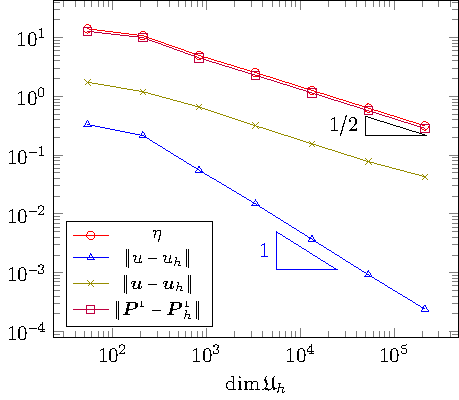
\includegraphics[width=15em]{plots_stokes.pdf}
        \caption{Manufactured solution $u(x,y)=\sin(\pi x)^2 \sin(\pi y)^2$, $\ff = -\Delta \curl u$, $\bu=\curl u$ }
        \label{fig:enter-label}
    \end{figure}
Let $h \simeq \dim \UU_h^{-1/2}$
\begin{align*}
    \|u-u_h\|_\Omega = \cO(h^2), \quad \|\bu-\bu_h\|_\Omega = \cO(h), \quad \|\PP^\perp-\PP_h^\perp\| = \cO(h).
\end{align*}
\end{frame}
%%%%%%%%%%%%%%%%%%%%%%%%%%%%%%%%%%%%%%%%%%%%%%%%%
\begin{frame}{Lid-driven cavity flow}
Consider $\Omega =(0,1)^2$
    \begin{align*}
  u|_\Gamma = 0, \quad \partial_{\nn}u(x,y) = 
  \begin{cases}
    \phi(x) & \text{si} \quad  y=1, \\
    0 & \text{else},
  \end{cases}
\end{align*}

\begin{align*}
  \phi(x) = \begin{cases}
    1-\tfrac14\left(1-\cos(\tfrac{0.1-x}{0.1}\pi)\right)^2 & x\in[0,0.1], \\
    1 & x\in(0.1,0.9), \\
    1-\tfrac14\left(1-\cos(\tfrac{x-0.9}{0.1}\pi)\right)^2& x\in[0.9,1].
  \end{cases}
\end{align*}

\begin{align*}
  \bu(x,y)|_\Gamma = \begin{cases}
    (\phi(x),0)^\top & y=1, \\
    0 & \text{else}.
  \end{cases}
\end{align*}
\end{frame}
%%%%%%%%%%%%%%%%%%%%%%%%%%%%%%%%%%%%%%%%%%%%%%%%%%%%
\begin{frame}{ Lid-driven cavity flow}
\begin{figure}
  \begin{center}
  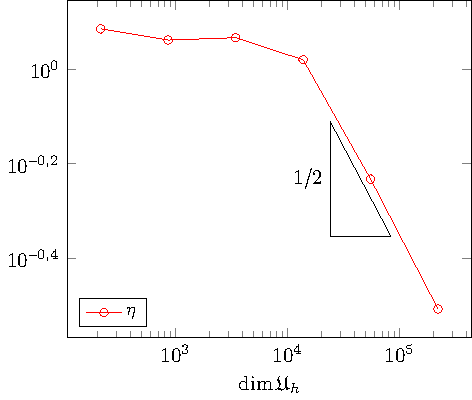
\includegraphics[width=0.35\textwidth]{plots_stokes2.pdf}
  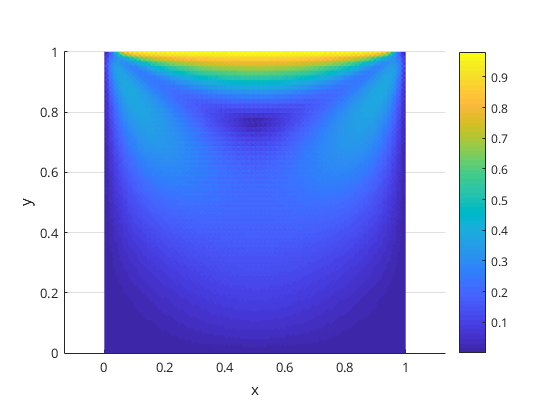
\includegraphics[width=0.35\textwidth]{LidDrivenVfield.png}
    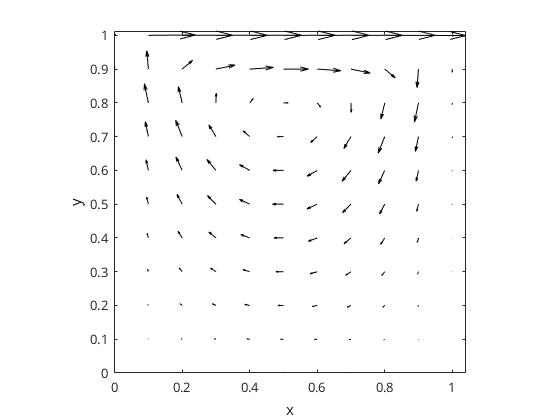
\includegraphics[width=0.35\textwidth]{LidDrivenVortexBig.png}
    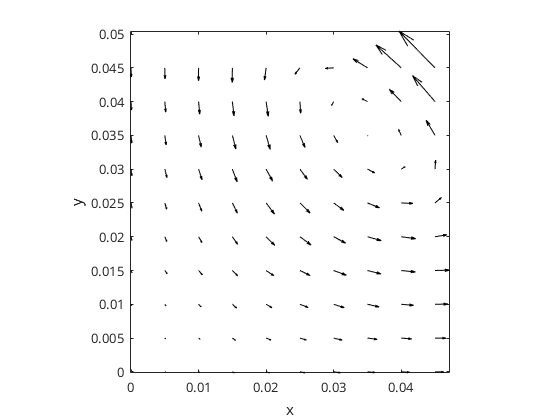
\includegraphics[width=0.35\textwidth]{LidDrivenVortexSmall.png}
  \end{center}
\end{figure}
\end{frame}
%%%%%%%%%%%%%%%%%%%%%%%%%%%%%%%%%%%%%
\begin{frame}{Flow in channel with backward step}
$\Omega=(0,10)\times (-1,1)\setminus [0,2]\times[-1,0]$ 
\begin{align*}
  \partial_{\nn} u|_\Gamma = 0, \quad
  u(x,y)|_\Gamma = \begin{cases}
    -\frac{(2y+1)(y-1)^2}6 & x=0, \\
    -\frac{(y-1)^2(y+2)}{24} & x=10, \\ 
    0 & y = 1, \\
    -\frac16 & \text{en otro caso}.
  \end{cases}
\end{align*}
\begin{align*}
  \bu(x,y)|_\Gamma = \begin{pmatrix}
  u_1(x,y) \\ 0\end{pmatrix}, 
  \quad u_1(x,y) = \begin{cases}
    y(1-y) & x=0, \\
    \frac{(y+1)(1-y)}8 & x=10, \\
    0 &\text{else}.
  \end{cases}
\end{align*}
\end{frame}
%%%%%%%%%%%%%%%%%%%%%%%%%%%%%%%%%%%%%%%%%
\begin{frame}{Flow in channel with backward step}
  \begin{figure}
      \centering
      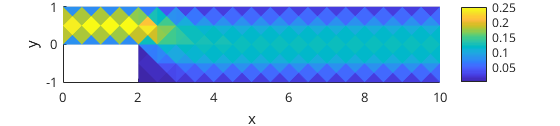
\includegraphics[width=0.65\textwidth]{StepVfield2.png}
      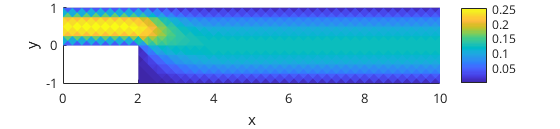
\includegraphics[width=0.65\textwidth]{StepVfield3.png}
      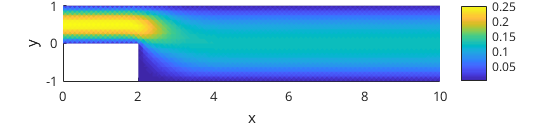
\includegraphics[width=0.65\textwidth]{StepVfield4.png}
      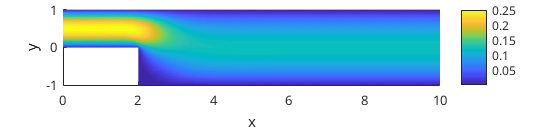
\includegraphics[width=0.65\textwidth]{StepVfield5.png}
      %\caption{Caption}
      \label{fig:enter-label}
  \end{figure}  
\end{frame}
%%%%%%%%%%%%%%%%%%%%%%%%%%%%%%%%%%%%%%
\begin{frame}{Singular solution}
    Singular solution, $\Omega=(0,1)^2$, $u(x,y)=|x-y|^\alpha \sin(\pi x)^2\sin(\pi y)^2$ with $\alpha = 2.01$
    \begin{figure}
        \centering
        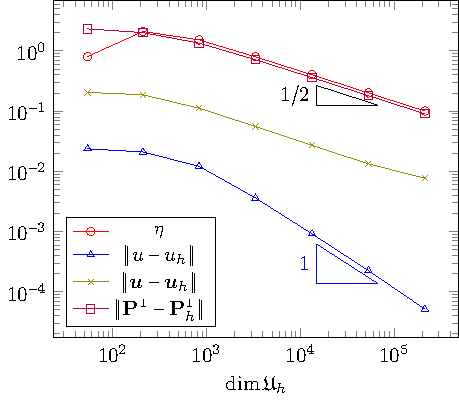
\includegraphics[width=0.5\textwidth]{plots_stokes3.pdf}
        \caption{Caption}
        \label{fig:enter-label}
    \end{figure}
\end{frame}


%%%%%%%%%%%%%%%%%%%%%%%%%%%%%%%%%%
\begin{frame}{References}
\begin{thebibliography}{99}
\bibitem{FHH23} T. Führer, P. Herrera and N. Heuer.
\newblock A DPG method for the quad-curl problem.
\newblock {\em Comput. Math. Appl.}, 149:221-238, 2023.

\bibitem{FHN19}
T. F\"uhrer, N. Heuer, and A. H. Niemi. 
\newblock An ultraweak formulation of the Kirchhoff–Love plate bending model
and DPG approximation. 
\newblock {\em Math. Comp.}, 88:1587--1619, 2019.

\bibitem{FH19} T. F\"uhrer and N. Heuer. 
\newblock Fully discrete DPG methods for the Kirchhoff–Love plate bending model. 
\newblock {\em Comput.
Methods Appl. Mech. Engrg.}, 343:550--571, 2019.


\bibitem{DG10} L. F. Demkowicz and J. Gopalakrishnan. 
\newblock A class of discontinuous Petrov–Galerkin methods. Part ii. optimal test functions.
\newblock {\em Numer. Methods Partial Differential Equations.}, 27 (1):70--105, 2011. 
 \end{thebibliography}
\end{frame}
\end{document}
